\section{Background \& Related Work}
\subsection{Model-Parallel Training}\label{sect:related_model_parallel}

Over the past decade, the deep learning community has developed several algorithms for training large neural networks. 
Most of them work by dividing the model between multiple workers, which is known as model parallelism. 
The exact way in which these algorithms divide the model determines their training performance and the maximum model size they can support.

\paragraph{Traditional model parallelism.} Historically, the first general strategy for training large models was to assign each device to compute a subset of each layer (e.g., a subset of neurons), then communicate the results between each other~\citep{alexnet,model_parallelism_survey1,model_parallelism_survey2}.
Since each device stores a fraction of layer parameters, this technique can train models with extremely wide layers that would not fit into a single GPU. However, applying traditional model parallelism to deep neural networks comes at a significant performance penalty, as it requires all-to-all communication after each layer.
As a result, while intra-layer parallelism is still widely used~\citep{meshtensorflow,zero}, it is usually applied within one physical server in combination with other strategies~\citep{krizhevsky2014oneweirdtrick,projectadam,beyond_data_and_model,megatron2}.

\vspace{-8pt}
\paragraph{Pipeline parallelism} circumvents the need for expensive all-to-all communication by assigning each device with one or several layers~\citep{huang2019gpipe}. During the forward pass, each stage applies its subset of layers to the inputs supplied by the previous stage, then sends the outputs of the last layer to the next stage. For the backward pass, this process is reversed, with each pipeline stage passing the gradients to the device that supplied it with input activations.

To better utilize the available devices, the pipeline must process multiple microbatches per step, allowing each stage to run in parallel on a different batch of inputs. In practice, the number of microbatches is limited by the device memory: this results in reduced device utilization when processing the first and the last microbatches, known as the ``bubble'' overhead~\citep{huang2019gpipe}. To combat this issue, subsequent studies propose using activation checkpointing, interleaved scheduling, and even asynchronous training~\citep{pipedream,megatron2,huang2019gpipe,shoeybi2019megatron,pipemare}.

Aside from model parallelism, there two more strategies for training large models: data parallelism with dynamic parameter loading~\citep{zero} and model-specific algorithms such as Mixture-of-Experts~\citep{shazeer2017outrageously}. We discuss these algorithms in Appendix~\ref{appendix:related} and compare the performance of offloading with SWARM in Section~\ref{appendix:training_throughput} and Appendix~\ref{appendix:equivalence}.

\vspace{-6pt}
\subsection{Distributed Training Outside HPC}
\label{sect:related_cost_efficent_collaborative}
\vspace{-2pt}

The techniques described in Section~\ref{sect:related_model_parallel} are designed for clusters of identical devices with rapid and reliable communication, making them a natural fit for the HPC setup. As we discussed earlier, such infrastructure is not always available, and a more cost-efficient alternative is to use ``preemptible'' instances~\citep{li2019speeding,zhang2020machine,proteus} or volunteer computing~\citep{volunteer_dl_async,hivemind_dmoe,eydle,dedloc}. However, these environments are more difficult for distributed training: each machine can disconnect abruptly due to a failure or preemption. Besides, since there is a limited number of available instances per region, training at scale often requires operating across multiple locations or using different instance types.

To handle unstable peers and heterogeneous devices, the research community has proposed elastic and asynchronous training methods, correspondingly.
Moreover, training large models over heterogeneous devices can be optimized with global scheduling~\cite{yuan2022decentralized}.
We describe these methods in more detail in Appendix~\ref{appendix:related}; importantly, neither of them are unable to satisfy all the constraints of our setup.

By contrast, the largest models have billions of parameters, which exceeds the memory limits of most low-end computers. 
However, model-parallel algorithms are not redundant, which makes them more vulnerable to hardware and network failures. 
There exist two methods that allow training large models with unreliable devices~\citep{hivemind_dmoe,thorpe2022bamboo}: however, the first one supports only specific architectures and requires at least 1Gb/s bandwidth, whereas the second one has no publicly available implementations, relies on redundant computations for fault tolerance and considers only the homogeneous setup.

\vspace{-6pt}
\subsection{Communication Efficiency and Compression}~\label{sect:related_communication_eficiency}
\vspace{-18pt}

In this section, we discuss techniques that address training with limited network bandwidth or high latency, such as gradient compression or overlapping computation with communication phases. These techniques are often necessary for distributed training without high-speed connectivity, because otherwise the performance of the system becomes severely bottlenecked by communication.

\vspace{-6pt}
\paragraph{Efficient gradient communication.}

Data-parallel training requires synchronization of gradients after each backward pass, which can be costly if the model has many parameters or the network bandwidth is limited. There exist several methods that approach this problem: for example, Deep Gradient Compression~\citep{deepgradientcompression} sparsifies the gradients and corrects the momentum after synchronization, while PowerSGD~\citep{vogels2019powersgd} factorizes the gradients and uses error feedback to reduce the approximation error.
Recently, \citet{wang2022finetuning} proposed to compress the changes of model activations, achieving high-speed communication for finetuning models of up to 1.5B parameters.
Alternatively, \citet{Dettmers20158BitAF} uses 8-bit quantization to compress gradients before communication. We evaluate it along with compression-aware architectures, leaving the exploration of more advanced approaches to future work.

Besides gradient compression, another effective technique is to use layer sharing~\citep{albert}, which reduces the number of aggregated gradients by a factor of how many times each layer is reused.

\paragraph{Overlapping communication and computation.}

Model, pipeline, and data parallelism all have synchronization points and require transfer of gradients or activations. One way to reduce the transfer cost is to overlap communication with computation, {\it hiding} the synchronization latency. This overlap can be achieved by combining parallelism techniques~\citep{krizhevsky2014oneweirdtrick, zero}, by synchronizing gradients layer-by-layer in lockstep with backpropagation~\citep{paszke2019pytorch}, or by using pure pipeline parallelism~\citep{huang2019gpipe,pipedream}.
However, pure pipeline parallelism requires many stages to effectively hide the latency. To overcome this problem, we study inter-layer compression techniques that work well even with relatively few pipeline stages.


\begin{figure*}[t]
    \centering
    \begin{minipage}[][][b]{0.64\textwidth}
    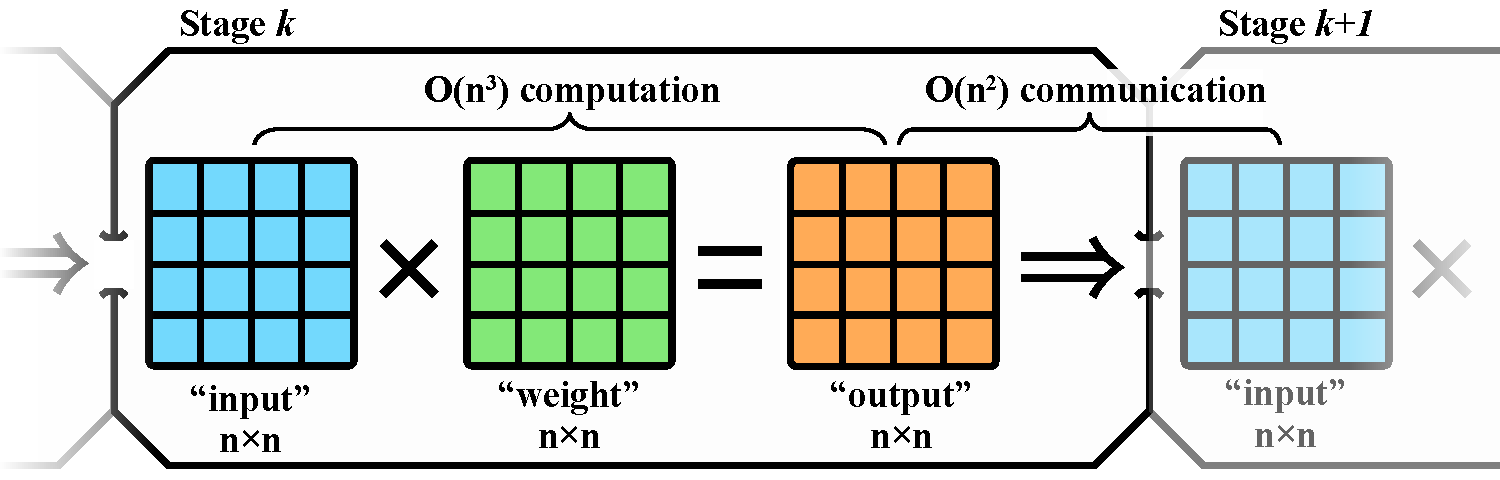
\includegraphics[width=\linewidth]{resources/squarecube_short_v2_max.pdf}
    \caption{\textbf{(Left)} An intuitive explanation of the square-cube law, \textbf{(Right)} Relative device utilization for Transformer layers using Tesla V100 and 500Mb/s network bandwidth. See Section~\ref{sect:experiments_square_cube} and Appendix~\ref{appendix:detailed_setup} for a detailed setup.}
    \label{fig:squarecube}
    \end{minipage}
    \begin{minipage}[][][b]{0.35\textwidth}
    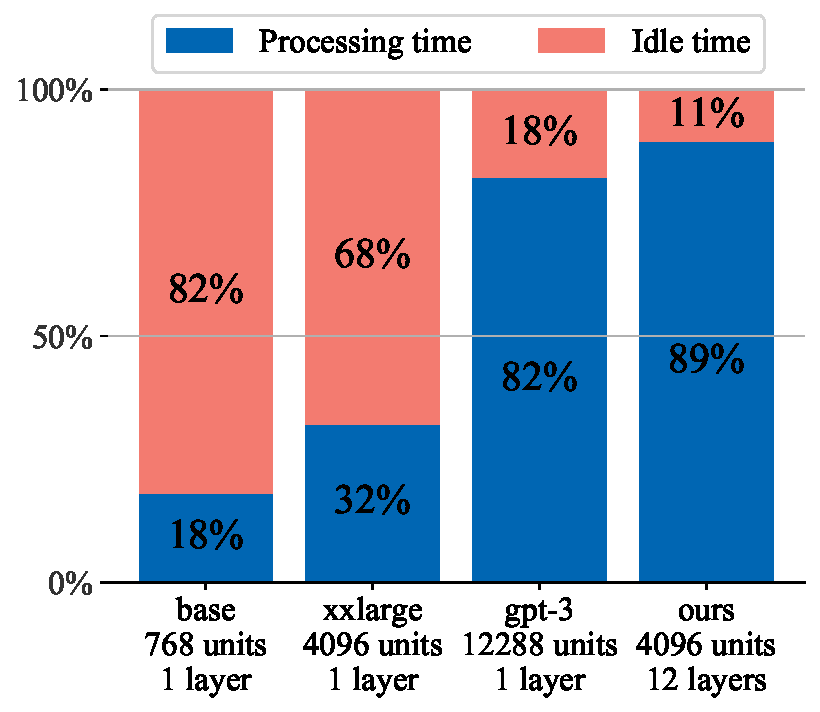
\includegraphics[width=\linewidth]{resources/perf_relative_notitle.pdf}
    \end{minipage}
    \vspace{-10pt}
\end{figure*}